\subsection{Columns}

\begin{figure}
  \begin{center}
  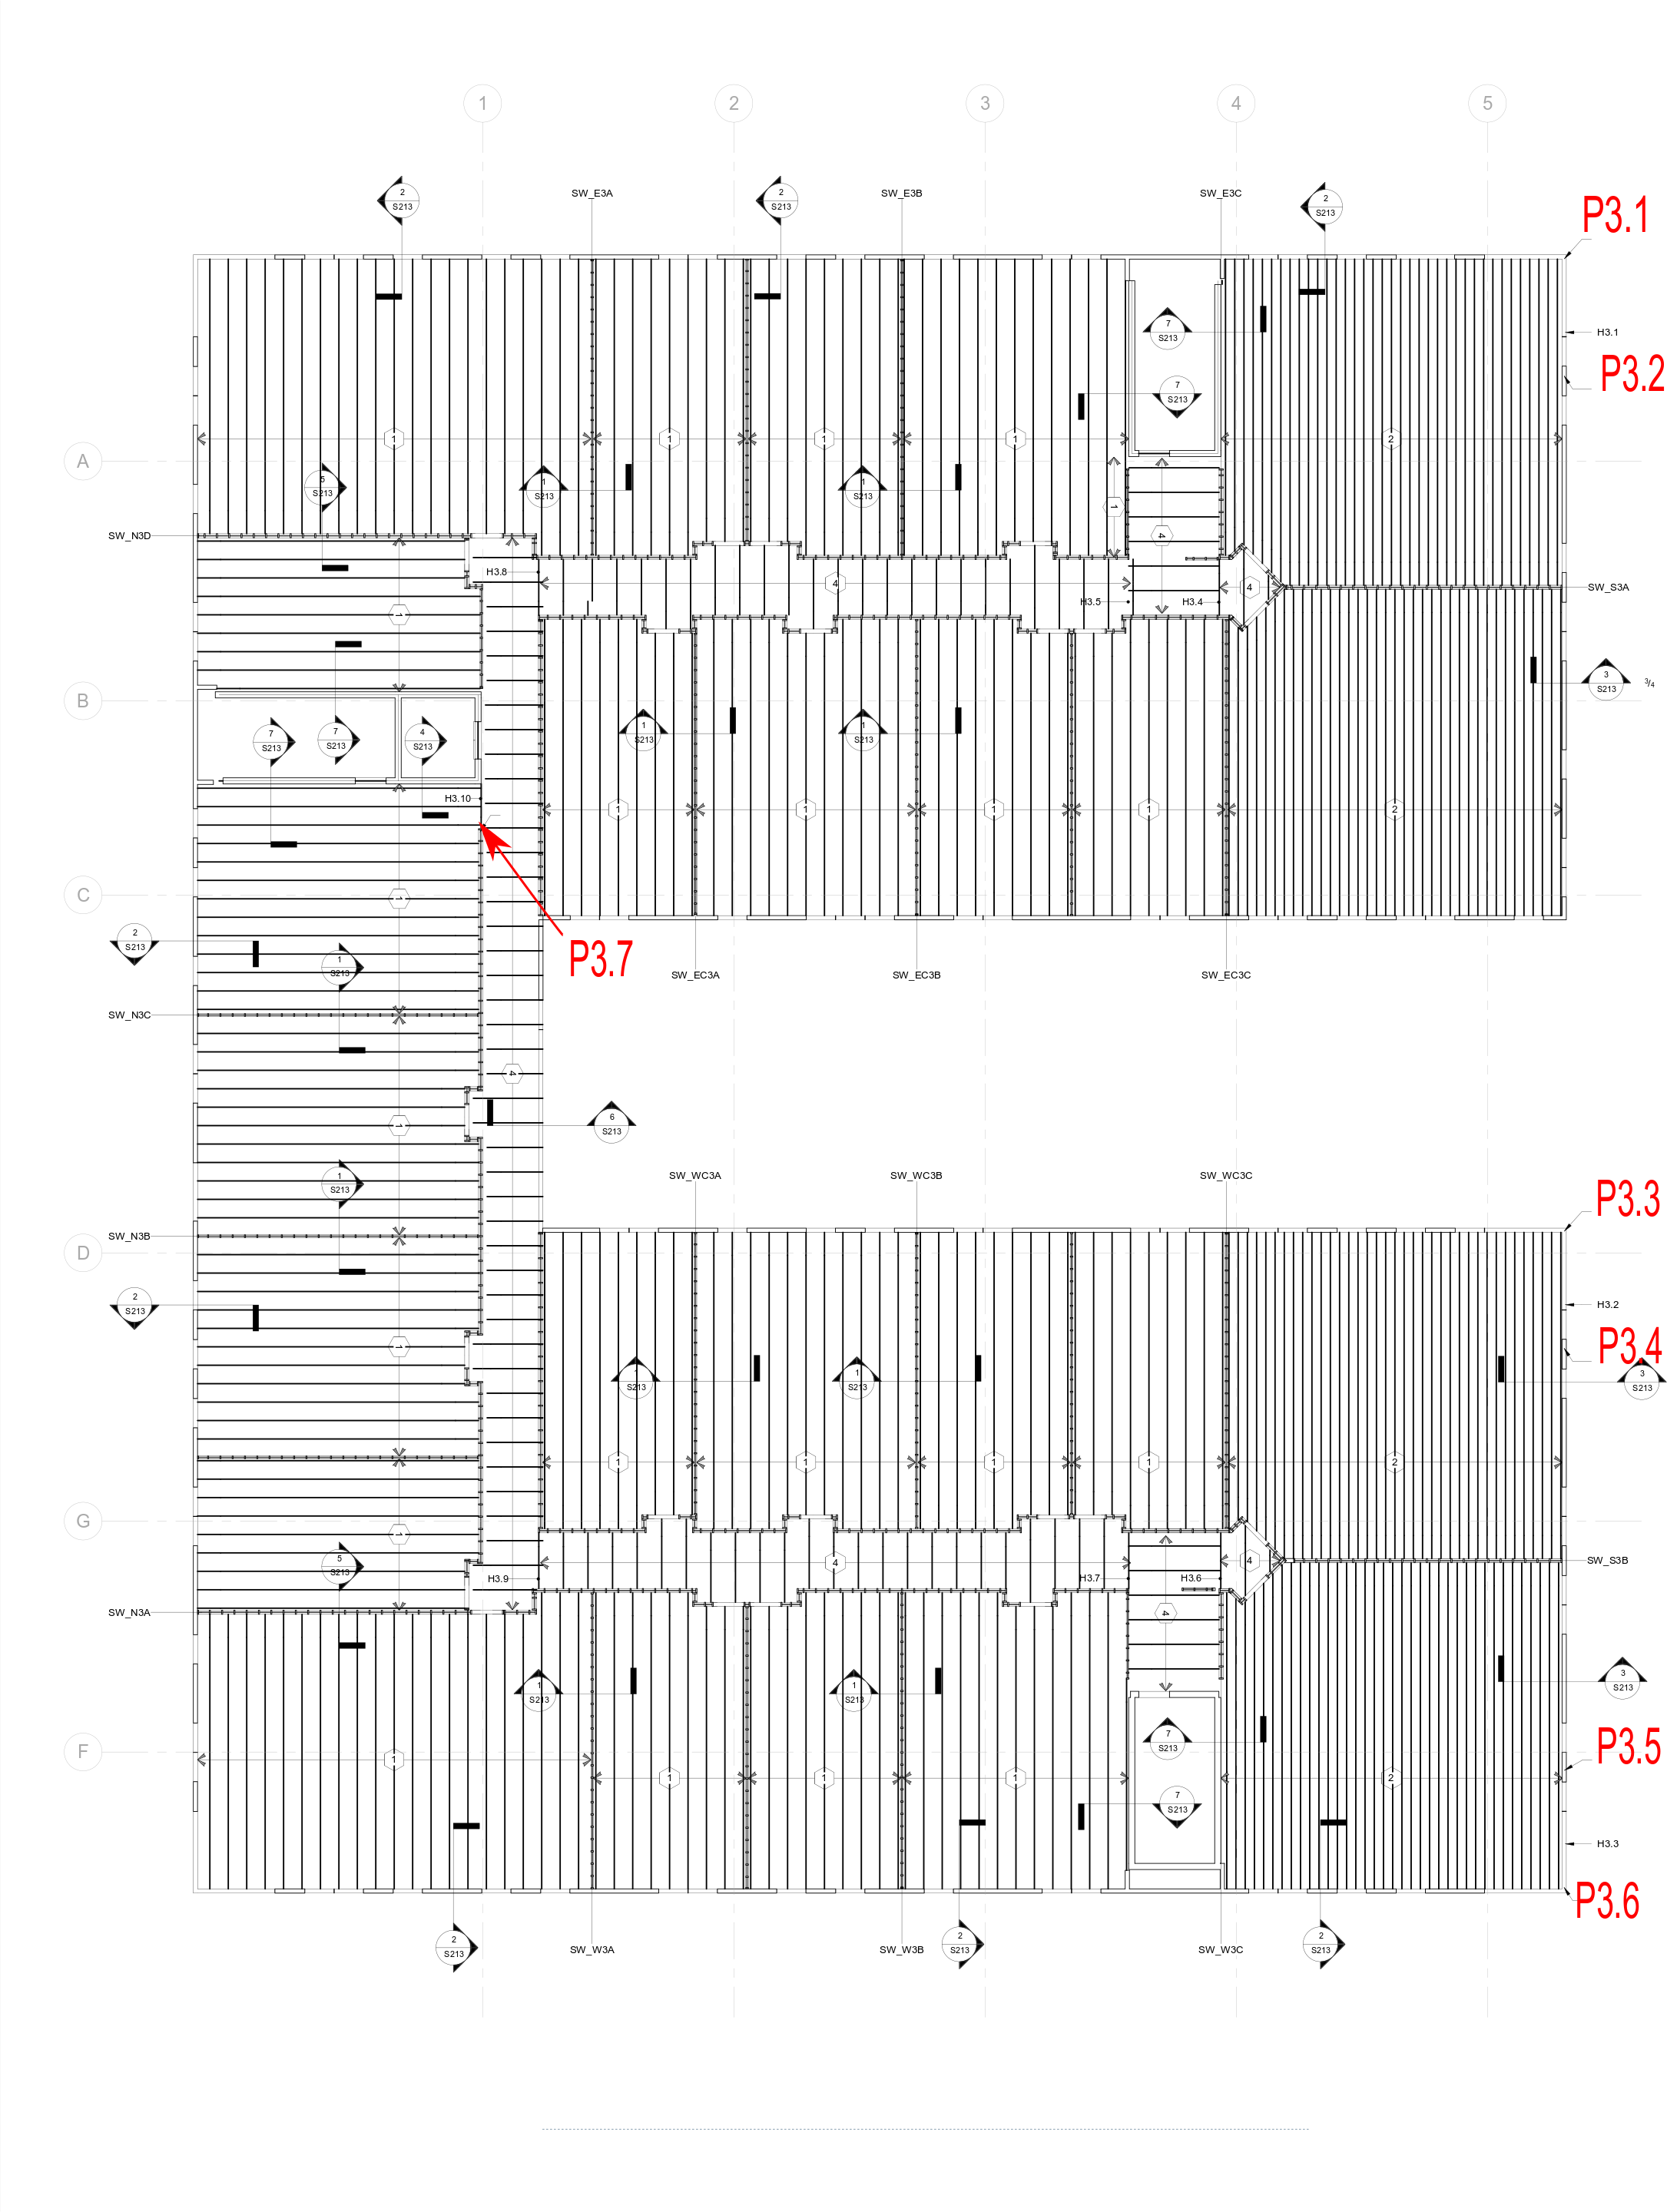
\includegraphics[width=120mm]{figures/columns_key_plan_roof}
  \end{center}
  \caption{Columns key plan. Roof}\label{fg_columns_key_plan_roof}
\end{figure}

\begin{figure}
  \begin{center}
  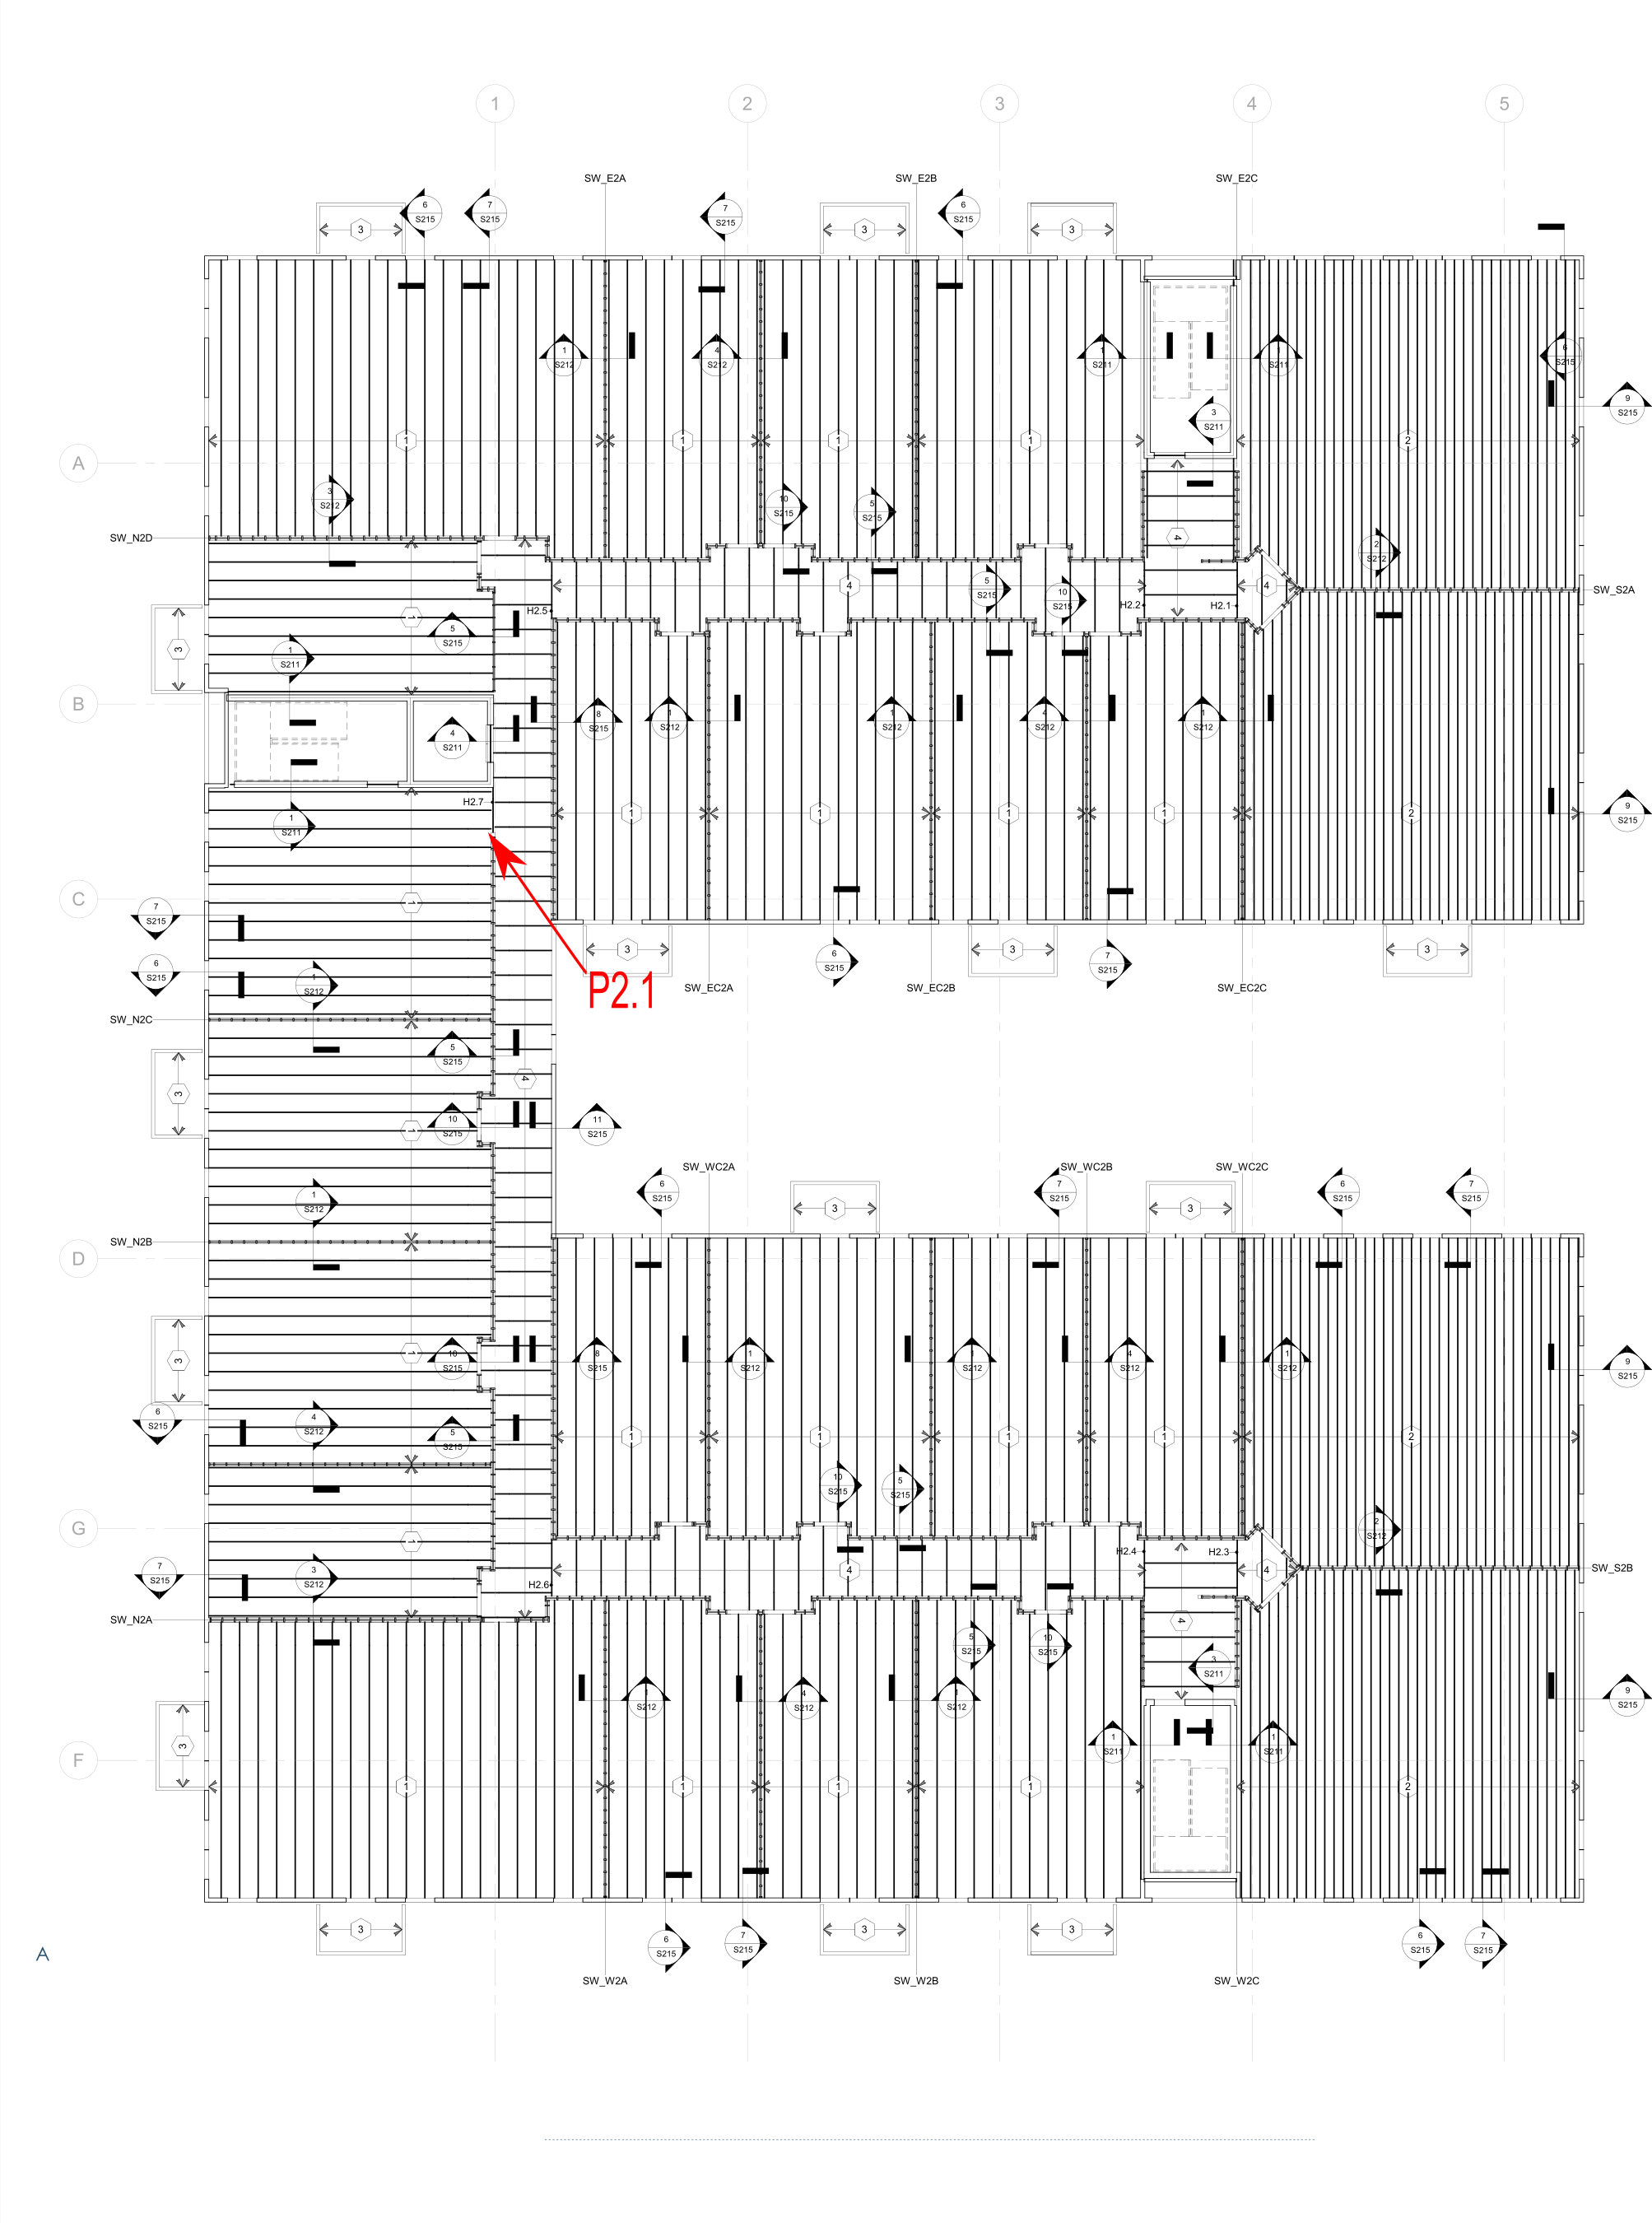
\includegraphics[width=120mm]{figures/columns_key_plan_3rd_floor}
  \end{center}
  \caption{Columns key plan. Third floor}\label{fg_columns_key_plan_3rd_floor}
\end{figure}

\begin{figure}
  \begin{center}
  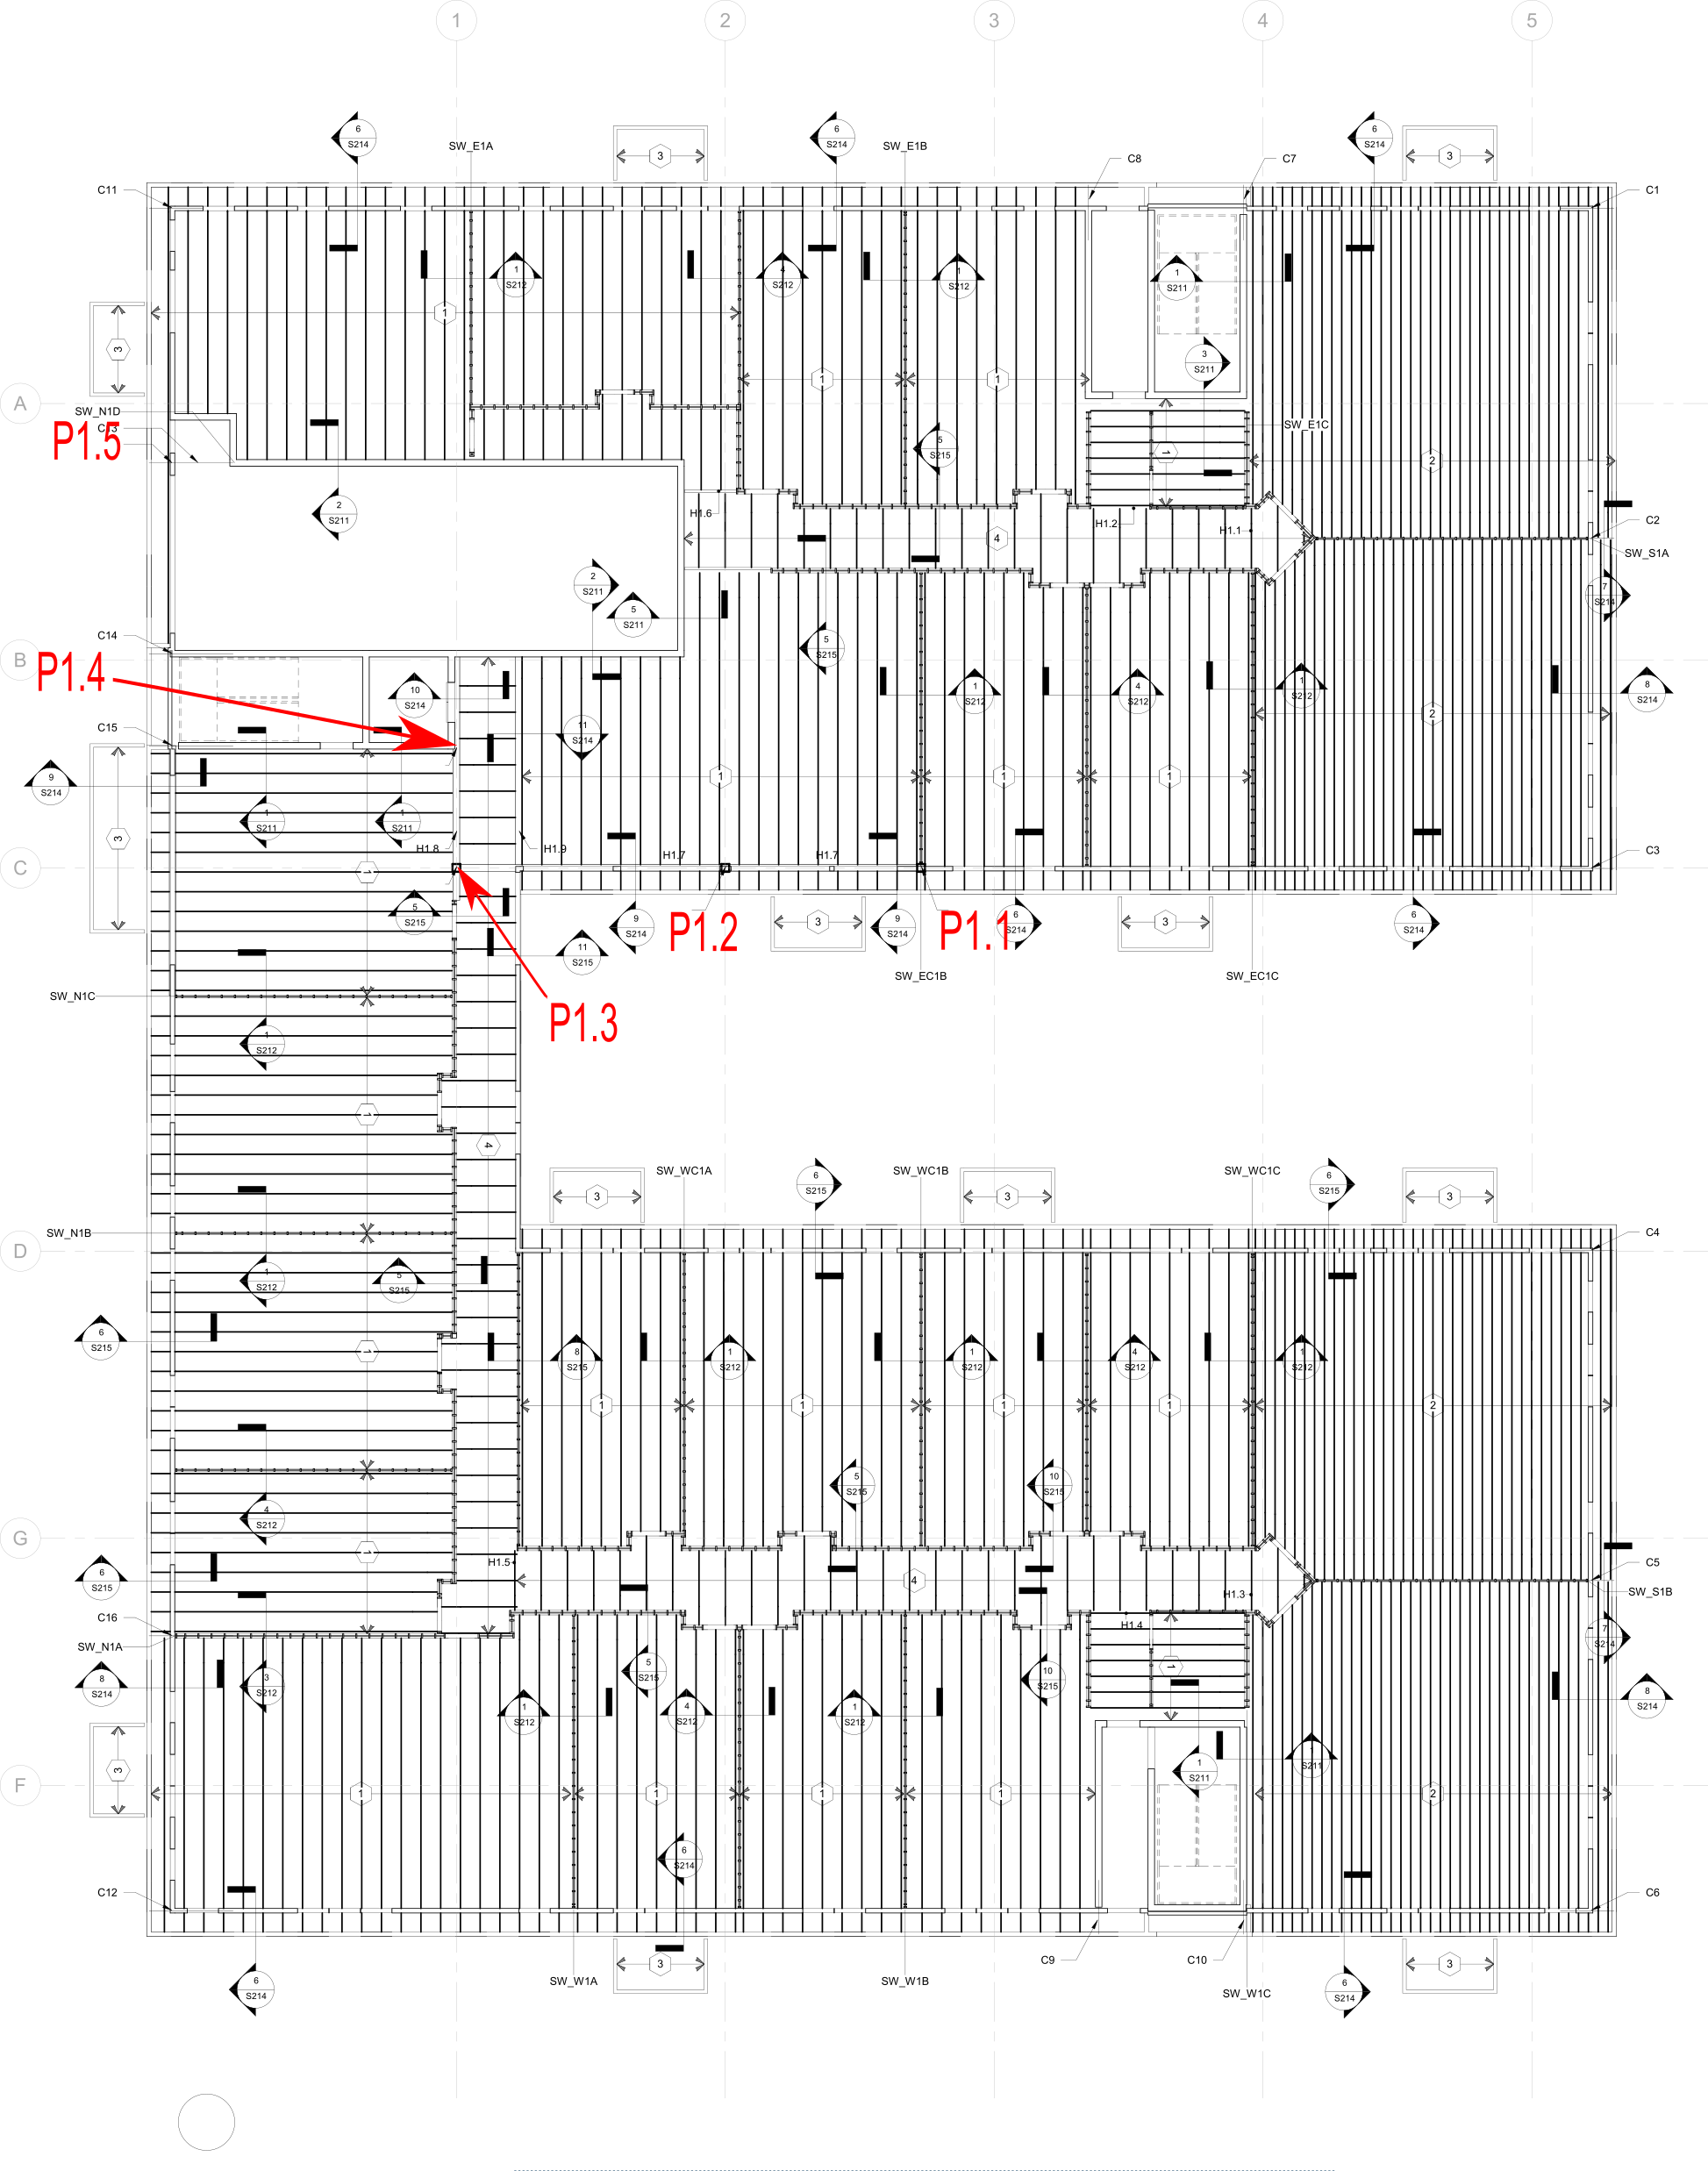
\includegraphics[width=120mm]{figures/columns_key_plan_2nd_floor}
  \end{center}
  \caption{Columns key plan. Second floor}\label{fg_columns_key_plan_2nd_floor}
\end{figure}

\subsubsection{Columns P3.1 to P3.6}

\paragraph{Loads.}

\begin{itemize}
\item Load from header: 4.8 kN
\end{itemize}

\paragraph{Internal forces.}

\noindent Maximum induced axial force:

\begin{equation}
  N_{max}= 4.8\ kN
\end{equation}

\paragraph{Compression check.}

\subparagraph{Mechanical properties}

\begin{itemize}
\item Species: Spruce-pine-fir No.2
\item $E_{min}= 2.55\ GPa$
\item $F_c= 2.93\ MPa$.
\item Sections dimensions: (6x6''), effective (5.5x5.5'')= 139.7 x 139.7  mm.
\item Unbraced lenght x axis: 3.45 m
\item Unbraced lenght y axis: 2.59 m
\item Column stability factor: $C_P= 0.74$
\end{itemize}

\begin{equation}
  N'_s= 42.46\ kN
\end{equation}

\noindent Structural compression check: $N'_s = 42.46 > 4.8 = N_{max} \implies OK$

\subsubsection{Column P3.7}

\paragraph{Loads.}

\begin{itemize}
\item Load from header 3.10: 27.61 kN
\end{itemize}

\paragraph{Internal forces.}

\noindent Maximum induced axial force:

\begin{equation}
  N_{max}= 27.61\ kN
\end{equation}

\paragraph{Compression check.}

\subparagraph{Mechanical properties}

\begin{itemize}
\item Species: Douglas fir-Larch dense structural
\item $E_{min}= 4.27\ GPa$
\item $F_c= 9.31\ MPa$.
\item Sections dimensions: (4x6''), effective (3.5x5.5'')= 88.9 x 139.7  mm.
\item Unbraced lenght x axis: 2.902 m
\item Unbraced lenght y axis: 0.5 m
\item Column stability factor: $C_P= 0.64$
\end{itemize}

\begin{equation}
  N'_s= 74.34\ kN
\end{equation}

\noindent Structural compression check: $N'_s = 74.34 > 27.61 = N_{max} \implies OK$

\subsubsection{Column P2.1}

\paragraph{Loads.}

\begin{itemize}
\item Load from header 2.07 and post P3.10: 55.22 kN
\end{itemize}

\paragraph{Internal forces.}

\noindent Maximum induced axial force:

\begin{equation}
  N_{max}= 55.22\ kN
\end{equation}

\paragraph{Compression check.}

\subparagraph{Mechanical properties}

\begin{itemize}
\item Species: Douglas fir-Larch dense structural
\item $E_{min}= 4.27\ GPa$
\item $F_c= 9.31\ MPa$.
\item Sections dimensions: (4x6''), effective (3.5x5.5'')= 88.9 x 139.7  mm.
\item Unbraced lenght x axis: 2.902 m
\item Unbraced lenght y axis: 0.5 m
\item Column stability factor: $C_P= 0.64$
\end{itemize}

\begin{equation}
  N'_s= 74.34\ kN
\end{equation}

\noindent Structural compression check: $N'_s = 74.34 > 55.22 = N_{max} \implies OK$

\subsubsection{2x6 wood stud capacity}

\paragraph{Compression capacity.}

\subparagraph{Mechanical properties.}

\begin{itemize}
\item Species: Hem-fir stud select structural.
\item $E_{min}= 3.24\ GPa$
\item $F_c= 8.27\ MPa$.
\item Sections dimensions: (2x6''), effective (1.5x5.5'')= 38.1 x 139.7  mm.
\item Unbraced lenght x axis: 0.3 m
\item Unbraced lenght y axis: 3.45 m
\item Column stability factor: $C_P= 0.45$
\end{itemize}

\begin{equation}
  N'_s= 19.90\ kN
\end{equation}


\subsubsection{Columns P1.1, P1.2 and P1.3}
XXXX
